\documentclass[journal, a4paper]{IEEEtran}
\usepackage[italian]{babel}
\usepackage{booktabs}
\usepackage{siunitx}%Questo serve a caricare il pacchetto delle unità di misura del sistema internazionale%
\usepackage[utf8]{inputenc}
\usepackage{graphicx} 
\usepackage{url}
\usepackage{amsmath}
\usepackage{amssymb}


\usepackage{keyval}
\usepackage{xcolor}
\usepackage{caption}
\usepackage{subfig}
\usepackage{tikz}
\usepackage{circuitikz}
\usepackage{authblk}
%\usepackage{hyperref}

\begin{document}


% Define document title and author
	\title{Tecnologie Digitali - Logbook Week 101}
	\author[1]{Salvatore Bottaro}
		\author[2]{Lorenzo M. Perrone}
		\affil[1]{\texttt{salvo.bottaro@hotmail.it}}
		\affil[2]{\texttt{lorenzo.perrone.lmp@gmail.com}}
	\markboth{Tecnologie Digitali - Di Lieto}{}
	\maketitle
	
\begin{abstract}
	Logbook di laboratorio di Tecnologie Digitali, a.a. 2015/2016. Week 101
\end{abstract}

\section{Misura della velocità della luce}
Lo scopo principale dell'esperienza di questa settimana consiste nella misura della velocità della luce (in aria). L'apparato sperimentale a disposizione e il suo funzionamento è piuttosto intuitivo: un laser monocromatico a 660nm (la sua larghezza in lunghezza d'onda non è nota ma possiamo supporre che sia dell'ordine della decina di nm) funge da sorgente di una radiazione ben collimata che percorre un tratto di lunghezza determinata prima di essere riflessa da uno specchio e successivamente rilevata da un rivelatore. \\
Il laser viene controllato in corrente e la sua accensione segue un ciclo di frequenza di qualche centinaia di Herz, con un duty-cycle di pochi ns. Per mezzo di un oscilloscopio, è possibile visualizzare i segnali di accensione del laser e il picco del rivelatore: la distanza temporale fra i due picchi ci permette di ricavare il valore di \textit{c}, dividendo la lunghezza del cammino ottico per tale $\Delta T$. Per essere più precisi, ci potremmo aspettare - e in effetti è quello che si verifica - la presenza di un parametro non noto che si aggiunge sistematicamente all'intervallo di tempo misurato: questo parametro include un ritardo non facilmente determinabile fra l'impulso che triggera il laser e la sua effettiva accensione, stimato intorno ai 5 ns, più eventualmente delle lunghezze fisse ma difficilmente quantificabili date dalle dimensioni e dalla disposizione del rivelatore sul banchetto e in generale dell'apparato di produzione del segnale. Per questi motivi, è certamente consigliato eseguire un fit con più coppie $K_i - \Delta T_i$ e una funzione come la seguente:

\begin{equation}
\Delta T_i = \frac{K_i}{c} + cost.
\end{equation}

\section{Indice di rifrazione dell'acqua}
Oltre a misurare sperimentalmente la velocità della luce in aria, la seconda parte dell'attività consisteva nella misura dell'indice di rifrazione dell'acqua e in particolare a noi è stato chiesto di concentrarci su questo aspetto.\\
L'apparato sperimentale è esattamente lo stesso della misura di c, in più a nostra disposizione vi sono due tubi trasparenti cavi di PMMA, riempiti d'acqua, dalla lunghezza rispettivamente di 101(1)cm e di 202(1)cm. Un modo per misurare $n_a$ (indice di rifrazione dell'acqua) è quello di mantenere la lunghezza del cammino ottico totale $K$ fissa, e interporre lungo il percorso della radiazione luminosa le 4 combinazioni possibili dei due tubi, in modo da ottenere 4 diverse distanze $D_i$ percorse in acqua: 0m, 1m, 2m, 3m (valori approssimati). Con i rispettivi valori dei tempi di percorrenza $\Delta T_i$ è possibile anche questa volta eseguire un fit della funzione:

\begin{equation}
\Delta T_i = \frac{1}{c} \left[ K + (n_a - 1) D_i \right] + cost.
\end{equation}

Per accumulare quanti più dati possibili, abbiamo scelto di effettuare tre diverse serie di acquisizioni: le prime due con il metodo appena spiegato, vale a dire mantenendo fisso $K$ e variando $D$, la terza invece mantenendo fisso $D$ e variando $K$. Un'attenzione particolare è stata posta nella misura delle distanze K di ciascuna serie cercando, dove possibile, di quantificare al meglio l'esatta geometria del percorso ottico.\\

Per approfondire la questione: la costante parametro di fit nella precedente espressione può essere attribuita o al ritardo nel $\Delta T$ dell'oscilloscopio (come già spiegato), o ad un errore sistematico nel calcolo delle lunghezze K, o a entrambi i fattori. E' importante cercare di capire quale sia l'effetto prevalente poichè, se nelle prime due serie di dati per quanto riguarda il fit lasciare come parametro libero K o il ritardo nel $\Delta T$ è equivalente, dato che entrambi concorrono a modificare l'intercetta e non il coefficiente angolare della retta, che è il dato maggiormente interessante, nella funzione di fit della terza serie (come si vedrà) questo non è più vero: il valore dell'indice di rifrazione si estrae dall'intercetta, a cui concorre anche il ritardo $\Delta T$. Per questo motivo è necessaria una riflessione attenta sul ruolo di questi due parametri.\\
Una prima considerazione deriva dagli ordini di grandezza in gioco: alla scala dei tempi da noi usata sull'oscilloscopio si ha un'incertezza di 0.2 ns, che corrisponde ad una indeterminazione nelle lunghezze di circa 6cm. E' quindi più probabile che eventuali costanti additive siano determinate dal ritardo $\Delta T$, rispetto a degli errori sulle distanze, dal momento che questi ultimi dovrebbero essere dell'ordine delle decine di centimetri per diventare rilevanti. Ad esempio, scegliendo di fissare nel primo fit il $\Delta T = 5$ns e lasciando libero $K$, si ottiene uno scarto di più di 50cm rispetto al $K$ da noi misurato, ed è davvero molto poco probabile che questo corrisponda effettivamente a dei calcoli poco accurati di $K$. Se invece fissiamo $K$, otteniamo un $\Delta T \simeq 6.9 ns$. Analogamente, fissando $K$, dal secondo fit si può estrapolare un $\Delta T \simeq 6.1 ns$. Possiamo pensare che l'errore sul calcolo delle lunghezze sia della decina di cm e non maggiore.


% %Come riprova della bontà di questo valore, possiamo prendere la coppia D,T con D = 0m (cioè nell'aria) e inserendo il valore di \textit{c} noto otteniamo come $\Delta T$ circa 6.8 ns, compatibile con il risultato del fit.

\subsection{Prima serie}
Per le misure effettuate nella prima serie, è stata disposta la strumentazione come in Figura (\ref{fig:disegn_primaserie}). Nella tabella seguente, invece, vengono riportati i valori di $T_i$ e $D_i$.


\begin{table}
\centering
\begin{tabular}{l|l|l|l}
\hline
D(m) & $\Delta$D (m) & T(ns) & $\Delta$T (ns)\\
\hline
3.03 & 0.04 & 34.2 & 0.2 \\
2.02 & 0.02 & 33.4 & 0.2 \\
1.01 & 0.02 & 32.4 & 0.2 \\
0.00 & 0.01 & 31.2 & 0.2 \\
\hline
\end{tabular}
\end{table}
~\\

\begin{figure}
\centering
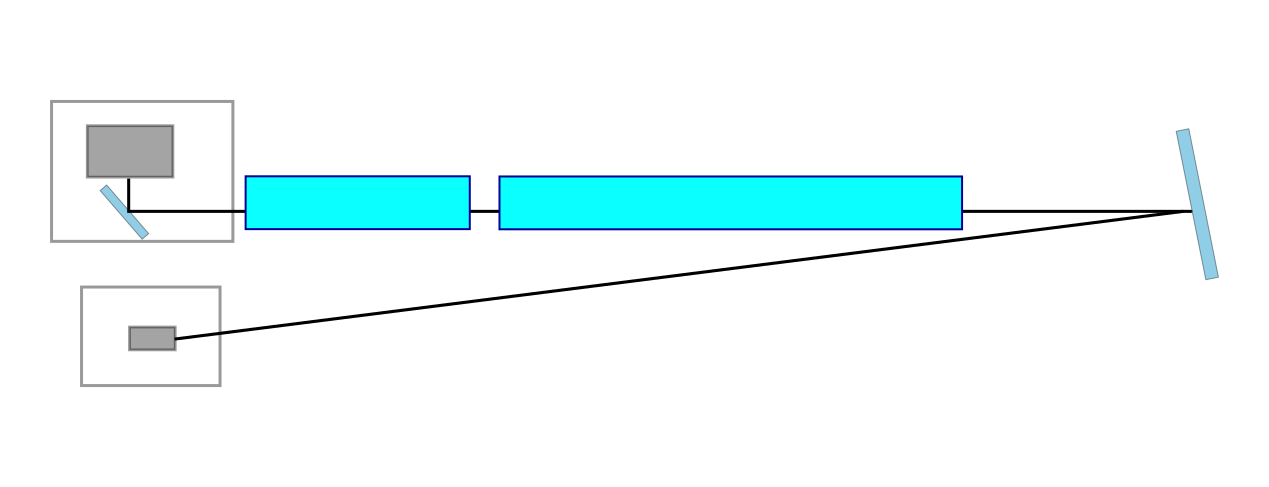
\includegraphics[width=0.9\linewidth]{./disegn_primaserie}
\caption{Disposizione della strumentazione per la prima serie di dati: la lunghezza totale del cammino ottico $K$ è fissa, cambiano le diverse combinazioni dei tubi.}
\label{fig:disegn_primaserie}
\end{figure}


Il risultato del fit è in Figura (\ref{fig:indice_primaserie_tret}): il valore di $n_a$ risulta di 1.30(2), molto vicino a quello aspettato di 1.33.

\begin{figure}
\centering
\includegraphics[width=0.9\linewidth]{./indice_primaserie_tret}
\caption{Fit prima serie: $\Delta T$ parametro di fit.}
\label{fig:indice_primaserie_tret}
\end{figure}

\subsection{Seconda serie}
Nella seconda serie è stata leggermente modificata la disposizione dei tubi, accorciando K e ponendo nelle varie configurazioni il tubo da 2m lungo il percorso di andata, e quello da 1m lungo il percorso di ritorno (si veda Figura ()).\\

\begin{figure}
\centering
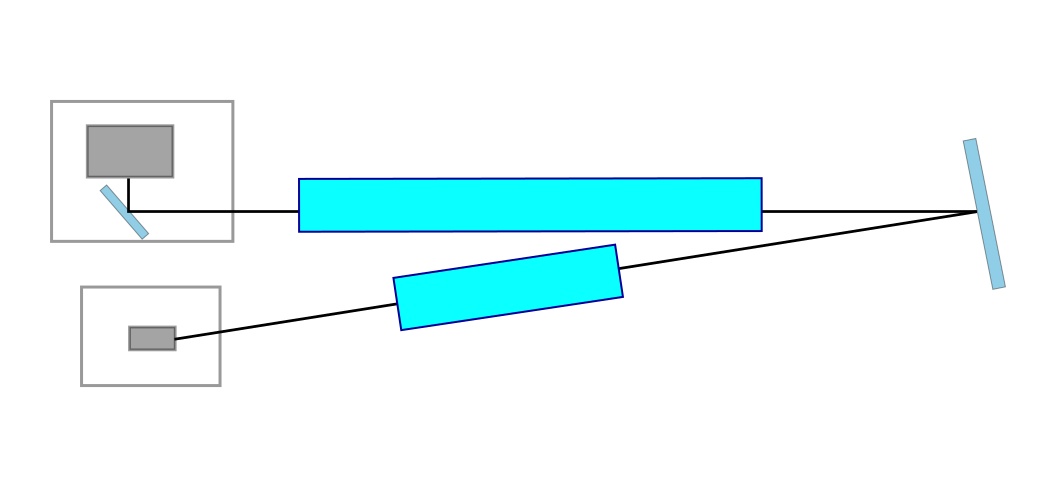
\includegraphics[width=0.9\linewidth]{./disegn_secondaserie}
\caption{Disposizione della strumentazione per la seconda serie di acquisizioni: i tubi sono disposti lungo il percorso di andata e ritorno. $K$ è fisso.}
\label{fig:disegn_secondaserie}
\end{figure}


I dati sono riportati nella tabella che segue:

\begin{table}
\centering
\begin{tabular}{l|l|l|l}
\hline
D(m) & $\Delta$D (m) & T(ns) & $\Delta$T (ns)\\
\hline
3.03 & 0.04 & 25.4 & 0.2 \\
2.02 & 0.02 & 24.6 & 0.2 \\
1.01 & 0.02 & 23.6 & 0.2 \\
0.00 & 0.01 & 22.8 & 0.2 \\
\hline
\end{tabular}
\end{table}
~\\

Il risultato del secondo fit è $n_a = 1.26(1)$, sensibilmente più distante dal valore di 1.33. Purtroppo, con soli 4 dati la pendenza della retta è modificata sostanzialmente al variare anche minimo di uno dei punti terminale, ad esempio.

\begin{figure}
\centering
\includegraphics[width=0.9\linewidth]{./indice_secondaserie_tret}
\caption{Fit seconda serie - $\Delta T$ parametro di fit}
\label{fig:indice_secondaserie_tret}
\end{figure}

Come ulteriore approfondimento, possiamo prendere in considerazione il fatto che il tubo contenente l'acqua è, come già detto, composto di PMMA, e in particolare vi è uno spessore di circa 1cm di tale materiale ad entrambe le estremità. Per questo motivo, in realtà alle distanze $D_i$ dovremmo sottrarre 0,2 o 4cm (in base a quale configurazione stiamo usando), e riaggiungere il prodotto di queste per l'indice di rifrazione del materiale, di 1.488. Come si può vedere da una veloce stima, tuttavia, il risultato di questa procedure introduce dei $\delta T$ dell'ordine del centesimo di ns, trascurabili rispetto all'errore dell'oscilloscopio.

\begin{equation}
\delta T = (n_{PMMA} - n_a)*\left\lbrace 0.02m, 0.04m\right\rbrace /c \simeq \left\lbrace 0.01, 0.02\right\rbrace ns
\end{equation}

\begin{figure}
\centering
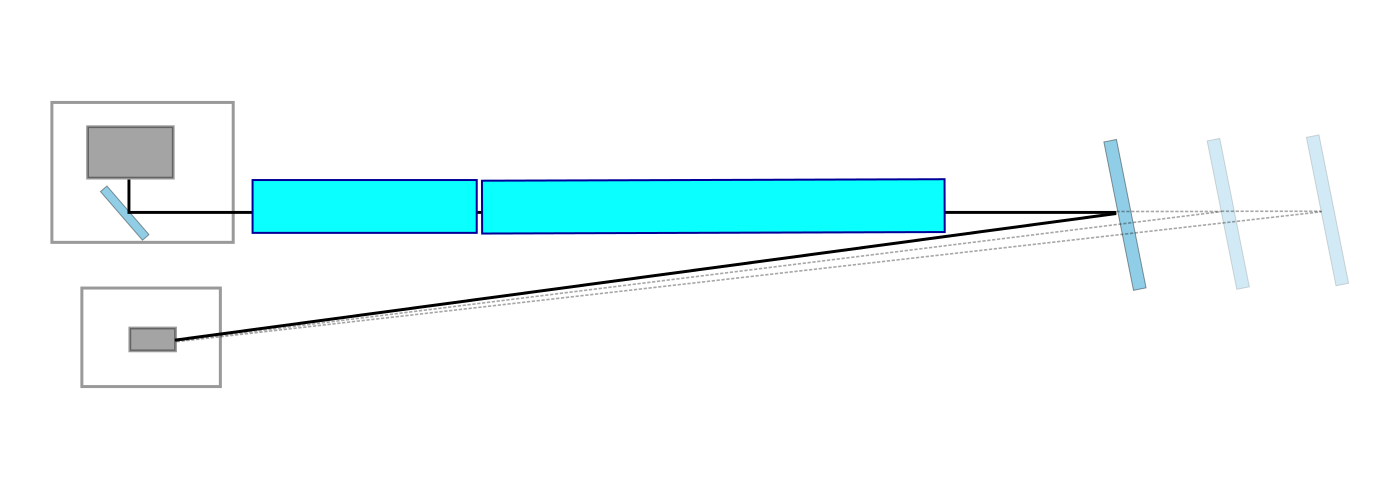
\includegraphics[width=0.9\linewidth]{./disegn_terzaserie}
\caption{Disposizione della strumentazione durante la terza serie di acquisizioni: entrambi i tubi sono presenti e fissati, varia $K$.}
\label{fig:disegn_terzaserie}
\end{figure}


\begin{thebibliography}{5}

	%Each item starts with a \bibitem{reference} command and the details thereafter.
	
	\bibitem{JH6} % Conference paper
	Product data sheet: Dual Type D Flip-Flop \textsc{mc14013b}.
	\url{http://onsemi.com}

	\bibitem{M06} % Conference paper
	Paul Horowitz, Winfield Hill - The Art of Electronics. Cambridge University Press (1989).
	
\end{thebibliography}


\end{document}